\begin{introduction}
    \item 向量
    \item 向量的运算
    \item 坐标表示
    \item 定比分点
\end{introduction}

\section{向量}

\begin{definition}[向量]
    既有大小又有方向的量称为向量。
\end{definition}

不同于之前研究的量，向量之间的关系更复杂：
\begin{enumerate}
    \item 相等：大小和方向都相等
    \item 平行或者说是共线：方向相等或者相反
\end{enumerate}

\begin{definition}[零向量与单位向量]
    特别地我们定义零向量：$\Vec{0}$是大小为$0$，方向任意的向量。此外我们定义长度为 $1$ 的向量为单位向量。
\end{definition}

\section{向量的运算}

\subsection{加减法和数乘}

\begin{multicols}{3}
    \begin{center}
        \begin{figure} [H]
            \centering
            \caption*{\textbf{加法：平行四边形定则}}
            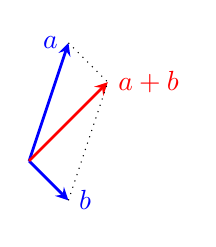
\begin{tikzpicture}[scale=0.5]
                \draw[line width=1pt,blue,-stealth](0,0)--(1,3) node[left]{$\boldsymbol{\Vec{a}}$};
                \draw[line width=1pt,blue,-stealth](0,0)--(1,-1) node[right]{$\boldsymbol{\Vec{b}}$};
                \draw[line width=1pt,red,-stealth](0,0)--(2,2) node[right]{$\boldsymbol{\Vec{a}+\Vec{b}}$};
                \draw[black,dotted](1,3)--(2,2);
                \draw[black,dotted](1,-1)--(2,2);
            \end{tikzpicture}
        \end{figure}
    \end{center}

    \columnbreak

    \begin{center}
        \begin{figure} [H]
            \centering
            \caption*{\textbf{减法：三角形定则}}
            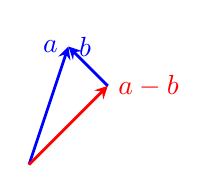
\begin{tikzpicture}[scale=0.5]
                \draw[line width=1pt,blue,-stealth](0,0)--(1,3) node[left]{$\boldsymbol{\Vec{a}}$};
                \draw[line width=1pt,blue,-stealth](2,2)--(1,3) node[right]{$\boldsymbol{\Vec{b}}$};
                \draw[line width=1pt,red,-stealth](0,0)--(2,2) node[right]{$\boldsymbol{\Vec{a}-\Vec{b}}$};
            \end{tikzpicture}
        \end{figure}
    \end{center}

    \columnbreak

    \begin{center}
        \begin{figure} [H]
            \centering
            \caption*{\textbf{数乘}}
            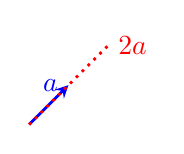
\begin{tikzpicture}[scale=0.5]
                \draw[line width=1pt,blue,-stealth](0,0)--(1,1) node[left]{$\boldsymbol{\Vec{a}}$};
                \draw[line width=1pt,red,dotted](0,0)--(2,2) node[right]{$\boldsymbol{\Vec{2a}}$};
            \end{tikzpicture}
        \end{figure}
    \end{center}
\end{multicols}

\subsubsection{向量的加法}

\begin{theorem}[向量加法]
    首尾相连，连连看！$\overrightarrow{AB} + \overrightarrow{BC} = \overrightarrow{AC}$
\end{theorem}

\begin{example}
    点 $O$ 是平行四边形 $A B C D$ 的两条对角线的交点，则 $\overrightarrow{A O}+\overrightarrow{O C}+\overrightarrow{C B}$ 等于 （\qquad）
    \begin{tasks}(4)
        \task $\overrightarrow{A B}$
        \task $\overrightarrow{B C}$
        \task $\overrightarrow{C D}$
        \task 0
    \end{tasks}
\end{example}

\v{6em}

\begin{example}
    如图，在正六边形 $A B C D E F$ 中， $\overrightarrow{B A}+\overrightarrow{C D}+\overrightarrow{F B}$ 等于 （\qquad）
    \begin{tasks}(4)
        \task $\overrightarrow{0}$
        \task $\overrightarrow{B E}$
        \task $\overrightarrow{A D}$
        \task $\overrightarrow{C F}$
    \end{tasks}
\end{example}
\begin{center}
    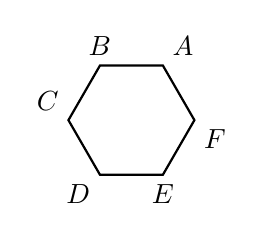
\begin{tikzpicture}[scale=0.8]
        % Define coordinates for the regular hexagon
        \foreach \i in {1,...,6} {
                \coordinate (v\i) at ({cos(60*\i)}, {sin(60*\i)});
            }

        % Draw the hexagon
        \draw[thick] (v1) -- (v2) -- (v3) -- (v4) -- (v5) -- (v6) -- cycle;

        % Add labels
        \node[above right] at (v1) {$A$};
        \node[above] at (v2) {$B$};
        \node[above left] at (v3) {$C$};
        \node[below left] at (v4) {$D$};
        \node[below] at (v5) {$E$};
        \node[below right] at (v6) {$F$};
    \end{tikzpicture}
\end{center}

\v{6em}

\begin{example}
    化简下列各式：
    \begin{enumerate}
        \item $\overrightarrow{A B}+\overrightarrow{B C}+\overrightarrow{C A}$ ；

        \item $\overrightarrow{A B} + \overrightarrow{M B} + \overrightarrow{B O} + \overrightarrow{O M}$ ；

        \item $\overrightarrow{O A}+\overrightarrow{O C}+\overrightarrow{B O}+\overrightarrow{C O}$ ；

        \item $\overrightarrow{A B}+\overrightarrow{C A}+\overrightarrow{B D}+\overrightarrow{D C}$.
    \end{enumerate}
    其中结果为 $\overrightarrow{0}$ 的个数是（\quad）
    \begin{tasks}(4)
        \task 1
        \task 2
        \task 3
        \task 4
    \end{tasks}
\end{example}

\v{2em}

\begin{example}
    化简下列各式：
    \begin{itemize}
        \item $\overrightarrow{A B}+\overrightarrow{B C}+\overrightarrow{C D}+\overrightarrow{D A}$ ；
        \item $\overrightarrow{A B}+\overrightarrow{D F}+\overrightarrow{C D}+\overrightarrow{B C}+\overrightarrow{F A}$ ；
        \item $(\overrightarrow{A B}+\overrightarrow{M B})+(\overrightarrow{B O}+\overrightarrow{B C})+\overrightarrow{O M}$.
    \end{itemize}
\end{example}

\begin{example}
    如图，已知点 $D$、$E$、$F$ 分别是 $\triangle A B C$ 三边 $A B
    $、$B C$、$C A$ 的中点，求证： $\overrightarrow{E A}+\overrightarrow{F B}+\overrightarrow{D C}=\overrightarrow{0}$.
\end{example}

\begin{tikzpicture}[scale=0.7]
    \coordinate (A) at (0,3);
    \coordinate (B) at (-2.5,0);
    \coordinate (C) at (2.5,0);

    \filldraw[black] (A) circle (1.5pt) node[above] {$A$};
    \filldraw[black] (B) circle (1.5pt) node[below] {$B$};
    \filldraw[black] (C) circle (1.5pt) node[below] {$C$};

    \draw (A) -- (B) -- (C) -- cycle;

    \coordinate (D) at ($(A)!0.5!(B)$);
    \coordinate (E) at ($(B)!0.5!(C)$);
    \coordinate (F) at ($(A)!0.5!(C)$);

    \filldraw[black] (D) circle (1.5pt) node[left] {$D$};
    \filldraw[black] (E) circle (1.5pt) node[below] {$E$};
    \filldraw[black] (F) circle (1.5pt) node[right] {$F$};

    \draw (D) -- (E) -- (F) -- cycle;
\end{tikzpicture}

\begin{theorem}[运算律]
    不难验证，这样定义的向量运算满足：
    \begin{multicols}{2}
        \begin{enumerate}
            \item 加法交换律：$\Vec{a}+\Vec{b} = \Vec{b}+\Vec{a}$
            \item 加法结合律：$\Vec{a}+(\Vec{b}+\Vec{c}) = (\Vec{a}+\Vec{b})+\Vec{c}$
            \item 加法有零元：$\Vec{a}+\Vec{0} = \Vec{a}$
                  \columnbreak
            \item 数乘向量分配律：$\lambda(\Vec{a}+\Vec{b}) = \lambda\Vec{a}+\lambda\Vec{b}$
            \item 数乘标量分配律：$(\lambda_1+\lambda_2)\Vec{a} = \lambda_1\Vec{a}+\lambda_2\Vec{a}$
            \item 数乘结合律：$\lambda_1 (\lambda_2\Vec{a}) = (\lambda_1\lambda_2)\Vec{a}$
            \item 数乘有单位元：$1 \Vec{a} = \Vec{a}$
        \end{enumerate}
    \end{multicols}
\end{theorem}

\begin{example}
    已知 $\vec{a}$、$\vec{b}$ 是不平行的向量，若 $\overrightarrow{A B}=\vec{a}+2 \vec{b}, \overrightarrow{B C}=-4 \vec{a}-\vec{b}, \overrightarrow{C D}=-5 \vec{a}-3 \vec{b}$ ，则下列关系中正确的是 （\qquad）
    \begin{tasks}(4)
        \task $\overrightarrow{A D}=\overrightarrow{C B}$
        \task $\overrightarrow{A D}=\overrightarrow{B C}$
        \task $\overrightarrow{A D}=2 \overrightarrow{B C}$
        \task $\overrightarrow{A D}=-2 \overrightarrow{B C}$
    \end{tasks}
\end{example}

\v{6em}

\subsection{内积}
内积也叫数量积。
\begin{definition}[内积]
    $$
        \overrightarrow{a}\cdot \overrightarrow{b} = |\overrightarrow{a}||\overrightarrow{b}|\cos \langle \overrightarrow{a},\overrightarrow{b} \rangle
    $$
    其中$\langle \overrightarrow{a},\overrightarrow{b} \rangle \in [0,\pi]$是两向量的夹角，$|\overrightarrow{a}|$是向量的模长。此外，规定任何向量和零向量的内积都是0。
\end{definition}

\begin{theorem}[内积的运算律]
    不难验证内积满足下列运算律：
    \begin{enumerate}
        \item 交换律：$\overrightarrow{a}\cdot \overrightarrow{b} = \overrightarrow{b} \cdot \overrightarrow{a}$
        \item 分配律：$\overrightarrow{a}\cdot (\overrightarrow{b}+\overrightarrow{c}) = \overrightarrow{a} \cdot \overrightarrow{b} + \overrightarrow{a} \cdot \overrightarrow{c}$
        \item 数乘结合律：$(\lambda \overrightarrow{a})\cdot \overrightarrow{b} = \lambda (\overrightarrow{a} \cdot \overrightarrow{b})$
    \end{enumerate}
\end{theorem}

\begin{example}
    已知 $|\vec{a}|=|\vec{b}|=1$ ，且 $\vec{a}$ 与 $\vec{b}$ 的夹角为 $\frac{\pi}{3}$ ，则 $\vec{b}$ 与 $\vec{a}+\vec{b}$ 的夹角为 （\qquad）
    \begin{tasks}(4)
        \task $\frac{\pi}{12}$
        \task $\frac{\pi}{6}$
        \task $\frac{7 \pi}{12}$
        \task $\frac{5 \pi}{6}$
    \end{tasks}
\end{example}

\v{6em}

\begin{example}
    已知两个单位向量 $\vec{a}, \vec{b}$ 满足 $|\vec{a}+3 \vec{b}|=3$ ，则 $\vec{a}, \vec{b}$ 夹角的余弦值为 （\qquad）
    \begin{tasks}(4)
        \task $-\frac{1}{6}$
        \task $-\frac{1}{3}$
        \task $\frac{1}{6}$
        \task $\frac{1}{3}$
    \end{tasks}
\end{example}

\v{6em}

\begin{example}
    已知向量 $\vec{a}$ ，$\vec{b}$ 满足 $|\vec{a}+\vec{b}|=2|\vec{a}-\vec{b}|$ ，则 $\sin \langle\vec{a}, \vec{b}\rangle$ 的最大值为 （\qquad）
    \begin{tasks}(4)
        \task $\frac{\sqrt{3}}{3}$
        \task $\frac{3}{5}$
        \task $\frac{\sqrt{2}}{2}$
        \task $\frac{4}{5}$
    \end{tasks}
\end{example}

\v{6em}

\subsection{投影}

\begin{definition}[投影]
    定义$\Vec{a}$在$\Vec{b}$上的投影为：
    $$
        \Vec{p} = \frac{|b|\cos \langle a,b \rangle}{|a|} \Vec{a}
    $$
\end{definition}

\section{向量的坐标表示}
直观地说，我们可以把向量放在平面直角坐标系坐标系中，在有大小方向的量和二元坐标之间建立一一对应的关系。

数学上，我们有向量基本定理：
\begin{theorem}
    如果$\Vec{e_1}, \Vec{e_2}$是平面内两个不共线的向量，那么该平面内任何一个向量都可以被他们俩\textbf{唯一地}线性表示：
    $$
        \Vec{a} = x\Vec{e_1} + y \Vec{e_2}
    $$
    我们称$\Vec{e_1}, \Vec{e_2}$是平面内的一组基。称二元组$(x,y)$是$\Vec{a}$在这组基下的坐标。

    特别地，如果它们的都是单位向量，并且夹角是$\pi / 2$，称为单位正交基。
\end{theorem}

\begin{example}
    已知向量 $\vec{a}, \vec{b}$ 满足 $|\vec{a}|=1, \vec{b}=(-1, \sqrt{2})$ ，且 $\vec{a}, \vec{b}$ 的夹角为 $\frac{\pi}{6}$ ，则 $|2 \vec{a}-\vec{b}|=$ （\qquad）
    \begin{tasks}(4)
        \task $\sqrt{2}$
        \task 1
        \task 2
        \task 4
    \end{tasks}
\end{example}

\v{6em}

\begin{theorem}[Cauchy不等式]
    $$
        -|\Vec{a}||\Vec{b}| \le \Vec{a} \cdot \Vec{b} \le |\Vec{a}||\Vec{b}|
    $$
    使用坐标表示则是：
    $$
        -\sqrt{x_1^2+y_1^2}\sqrt{x_2^2+y_2^2} \le x_1x_2 + y_1y_2 \le \sqrt{x_1^2+y_1^2}\sqrt{x_2^2+y_2^2}
    $$
    更一般的，实际上这个结论对$n$维向量都成立，这也就是我们之前证明的Cauchy不等式。
\end{theorem}

\subsection{定比分点}

\begin{theorem}[定比分点]
    设A、B不重合，C是直线AB上动点，并且
    $$
        \frac{AC}{AB} = \lambda
    $$
    那么
    $$
        \Vec{PC} = (1-\lambda) \Vec{PA} +   \lambda \Vec{PB}
    $$
\end{theorem}

\begin{figure}[H]
    \centering
    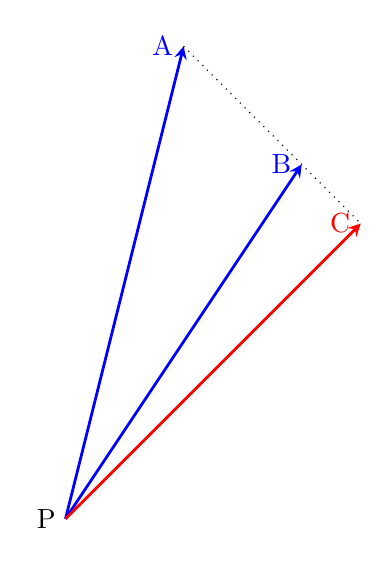
\begin{tikzpicture}[scale=1.5]
        \draw[line width=1pt,blue,-stealth](0,0)--(1,4) node[left]{$\mathrm{A}$};
        \draw[line width=1pt,blue,-stealth](0,0)--(2,3) node[left]{$\mathrm{B}$};
        \draw[line width=1pt,red,-stealth](0,0)--(2.5,2.5) node[left]{$\mathrm{C}$};
        \draw[black,dotted](1,4)--(2.5,2.5);
        \draw (0,0) node[left]{$\mathrm{P}$};
    \end{tikzpicture}
    \caption{$\lambda > 1$}
\end{figure}
这是前述的向量基本定理的一个应用。A、B不重合的条件下，PA、PB显然构成一组基，那么PC一定可以用PA、PB线性表示，而这个定理给出了该表示的坐标。

\subsection{三角形五心的向量表示}
以下设$a,b,c$是三角形ABC的三边长。O是三角形所在平面的一点。

\begin{theorem}
    O是外心$\iff |\Vec{OA}| = |\Vec{OB}| = |\Vec{OC}|$
\end{theorem}
\begin{proof}
    这是显然的，OA、OB、OC就是外接圆半径，长度自然相等。
\end{proof}

\begin{theorem}
    O是重心$\iff \Vec{OA} + \Vec{OB} + \Vec{OC} = \Vec{0}$
\end{theorem}
\begin{proof}
    设M是AB中点，根据定比分点，$\Vec{OA} + \Vec{OB} = 2 \Vec{OM}$，结合我们的条件也就是：
    $$
        2 \Vec{OM} = -\Vec{OC}
    $$
    也就是说O是CM的靠近M的三等分点，这显然就是重心。
\end{proof}
\begin{theorem}
    O是垂心$\iff \Vec{OA} \cdot \Vec{OB} = \Vec{OA} \cdot \Vec{OC} = \Vec{OC} \cdot \Vec{OB}$
\end{theorem}
\begin{proof}
    这是显然的：
    $$
        \Vec{OA} \cdot \Vec{OB} = \Vec{OA} \cdot \Vec{OC} \iff \Vec{OA} \cdot \Vec{CB} = 0 \iff OA \perp CB
    $$
\end{proof}
\begin{theorem}
    O是内心$\iff a\Vec{OA} + b\Vec{OB} + c\Vec{OC} = \Vec{0}$
\end{theorem}
\begin{proof}
    $\impliedby$：这是比较容易的

    $$
        \begin{aligned}
                     & a\Vec{OA} + b\Vec{OB} + c\Vec{OC} = \Vec{0}                          \\
            \implies & (a+b+c)\Vec{OA} +b\Vec{AB}+c\Vec{AB} = \Vec{0}                       \\
            \implies & \Vec{AO} = \frac{1}{a+b+c}(b\Vec{AB}+c\Vec{AC})                      \\
            \implies & \Vec{AO} = \frac{bc}{a+b+c}(\frac{1}{c}\Vec{AB}+\frac{1}{b}\Vec{AC})
        \end{aligned}
    $$
    其中
    $$
        \frac{1}{c}\Vec{AB}, \quad \frac{1}{b}\Vec{AC}
    $$
    分别是AB、AC方向的单位向量，根据平行四边形定则（这里由于都是单位向量，因此是一个菱形），它们相加得到的AO就一定在角平分线上了。

    $\implies$：这就不那么显然了。

    我们首先介绍两个引理
    \begin{lemma}[角平分线]
        在三角形ABC中，D在BC上，设AD是角A的平分线，那么：
        $$
            \frac{DB}{DC} = \frac{c}{b}
        $$
        此引理使用正弦定理很容易证明。
    \end{lemma}
    \begin{lemma}[内心]
        在三角形ABC中，D在BC上，设AD是角A的平分线，O是内心那么：
        $$
            \frac{OD}{OA} = \frac{a}{b+c}
        $$
        此引理使用正弦定理很容易证明。
    \end{lemma}
    那么我们就有
    $$
        \begin{aligned}
                     & a\Vec{OA} + b\Vec{OB} + c\Vec{OC}                    \\
            \implies & a\Vec{OA} +b(\Vec{OD}+\Vec{DB})+c(\Vec{OD}+\Vec{DC}) \\
            \implies & a\Vec{OA} + (b+c)\Vec{OD} + b\Vec{DB}+c\Vec{DC}
        \end{aligned}
    $$
    根据第一个引理
    $$
        b\Vec{DB}+c\Vec{DC} = \Vec{0}
    $$
    根据第二个引理
    $$
        a\Vec{OA} + (b+c)\Vec{OD} = \Vec{0}
    $$
    至此原命题证毕。
\end{proof}
\begin{theorem}
    O是关于A的旁心$\iff a\Vec{OA} = b\Vec{OB} + c\Vec{OC}$
\end{theorem}
\begin{proof}
    证明不做要求
\end{proof}